\documentclass[a4paper]{tufte-book}
\usepackage[utf8]{inputenc}
\hypersetup{colorlinks}% uncomment this line if you prefer colored hyperlinks (e.g., for onscreen viewing)

\title{Big Data, Statistical Learning}
\author{Julien Barrier}
\publisher{ESPCI Paris}
\newcommand{\thetitle}{Introduction to Big Data}
\newcommand{\theauthor}{Julien Barrier --- class of 2018}
\newcommand{\pc}{ESPCI Paris}
\newcommand{\thesubtitle}{Statistical \& Machine Learning}

\usepackage{microtype}
\usepackage{textcase}
\usepackage{booktabs}
\usepackage{tabularx}
\newcolumntype{R}{>{\raggedleft\arraybackslash}X}

\usepackage{graphicx}
\setkeys{Gin}{width=\linewidth,totalheight=\textheight,keepaspectratio}
\graphicspath{{graphics/}}

\usepackage{fancyvrb}
\fvset{fontsize=\normalsize}

\newcommand{\hangp}[1]{\makebox[0pt][r]{(}#1\makebox[0pt][l]{)}}

\newcommand{\hangstar}{\makebox[0pt][l]{*}}

\usepackage{xspace}

\newcommand{\monthyear}{%
\ifcase\month\or January\or February\or March\or April\or May\or June\or
July\or August\or September\or October\or November\or
December\fi\space\number\year
}

\newcommand{\openepigraph}[2]{%
%\sffamily\fontsize{14}{16}\selectfont
\begin{fullwidth}
\sffamily\large
\begin{doublespace}
\noindent\allcaps{#1}\\% epigraph
\noindent\allcaps{#2}% author
\end{doublespace}
\end{fullwidth}
}

\newcommand{\blankpage}{\newpage\hbox{}\thispagestyle{empty}\newpage}

\usepackage{units}
\usepackage{siunitx}
\usepackage{stmaryrd}
\usepackage{amsmath,amsfonts,amssymb}
\usepackage{mathrsfs}

\newcommand{\measure}[3]{#1/#2$\times$\unit[#3]{pc}}

\newcommand{\hlred}[1]{\textcolor{Maroon}{#1}}% prints in red
\newcommand{\hangleft}[1]{\makebox[0pt][r]{#1}}
\newcommand{\hairsp}{\hspace{1pt}}% hair space
\newcommand{\hquad}{\hskip0.5em\relax}% half quad space
\newcommand{\TODO}{\textcolor{red}{\bf TODO!}\xspace}
\newcommand{\ie}{\textit{i.\hairsp{}e.}\xspace}
\newcommand{\eg}{\textit{e.\hairsp{}g.}\xspace}
\newcommand{\na}{\quad--}% used in tables for N/A cells
\newcommand{\E}{\mathrm{E}}
\newcommand{\var}{\mathrm{Var}}
\newcommand{\cov}{\mathrm{Cov}}

% Generates the index
\usepackage{makeidx}
\makeindex

\usepackage{titlesec,titletoc}
\usepackage{multirow}

\begin{document}
\frontmatter

\thispagestyle{empty}
\begin{fullwidth}
    \setlength{\parindent}{0pt}
    \begin{center}
        \fontsize{24}{24}\selectfont\textit{
            \includegraphics*[width=2.6in]{ESPCI_baseline_couleur}
        }
    \end{center}
    \vspace{3in}\fontsize{36}{54}\selectfont\thetitle

    \vspace{0.125in}\fontsize{18}{18}\selectfont\thesubtitle

    \vfill\fontsize{14}{14}\selectfont\textit{\theauthor}
\end{fullwidth}

\newpage

\cleardoublepage
\chapter*{Introduction}

I have spartialed writing this handout from the notes I have taken from Olivier Rivoire's course on
Big Data and Statistical learning at \pc{} from May to April 2018. 
Please be considerate if some mistakes crop up in this work.

\emph{Julien}
\vspace{1cm}

Some book reading is advised during the course, partialicularly:

\begin{itemize}
    \item \emph{The Elements of Statistical Learning}, T.~Hastie, R.~Tibshirani and J.~Friedman, Springer Series in Statistics, 2008;
    \item \emph{Information Theory, Inference, and Learning Algorithms}, D.J.C.~MacKay, Cambridge University Press, 2003.
\end{itemize}

\vspace{1cm}

\textbf{Dr Olivier Rivoire}\\
Center for Interdisciplinary Research in Biology (CIRB)\\
Collège de France\\
olivier.rivoire@college-de-france.fr\\

\section*{Applications}

There are plenty of applications for Big Data problems. A few examples may be given:
\begin{description}
    \item[Post] learn + identify digits on enveloppes
    \item[Biology] DNA sequencing
    \item[IT] Face recognition
    \item[etc.]
\end{description}

Big Data is an issue of growing importance. As engineers, we may be familiar with such concepts.
\section*{Idea of marchine learning} 

The main idea of machine learning is to find models to give prediction of input data.
In facts, Big Data models are deduced from a training batch of N input-output
data, on which programs train to generalise models.
The deduced model \emph{input i} $\rightarrow$ \emph{output i} can then be
generalised to give prediction from a random input, as long as it relates to 
the training batch.



Analyticall, let's spartial with a collection of $x$ and $y$ data, where $x$ stands
for the input data and $y$ is the vector of the output data.
Each sample is going to have multiple dimensions, therefore we may use an
algebraic model. Let $N$ be the number of samples used and p the dimension of
each $x$ data. We may write x as an $N,p$ matrix and $y$ as a vector of $p$
dimensions.

We now N samples of p dimensions $x_{ij}$ associated with the N output data $y_i$.

From now on there are two possible cases: $y_i$ can be known or unknown.
In the fist case ($y_i$ known), the problem is said to be \emph{supervised}.
Hence we may work with a finite discrete set of data: $y_i = 1, \cdots, K$.
This problem is called categorical, and we can solve it with 
\emph{classification}.
We may also work with an infinite set of numbers: $y_i \in \mathbb{R}$. This
problem is called quantitative, and we can solve it with \emph{regression}.

The second case ($y_i$ unknown) is said to be \emph{unsupervised} and can be
solved via \emph{clustering} or \emph{dimension reduction} methods.

\section*{Deep learning}

In the past few years, there have been huge progress in the \emph{deep learning}
approach. It is based on so-called neurol networks, that are models inspired
by the brain operation.

People are trying to understand how to train these networks. It has had
remarkable outcomes in image recognition, social network filtering, medical
diagnoses, etc.

Deep learning is based on hidden layers, placed inbetween input and output layers
, that are trained to find correlations and mathematical models.

The goal of this course is to explain whate these objects are, how do they work,
and put it in relation with state of thepartial research.

What kind of open problems are there? How do neural networks operate? What are
their unsuperised learning behaviour?


\tableofcontents\thispagestyle{empty}

\mainmatter

\chapter{Least square regression, from small to big data}
\label{ch:least-square}

\section{Linear Regression at One Dimension}

Let $p =1$. If we work with N points, then $i=1,\cdots,N$, and we work with a
set of data $(x_i,y_i)$.

The goal here is to make a prediction of what the $y$ data should be when $x$ is
given.

The simplest possible model is the linear regression given by the equation 
\ref{linear1D}.
\begin{equation}
    y=\alpha + \beta x.
    \label{linear1D}
\end{equation}
Here, the main issue is to get the best $\alpha$ and $\beta$ for a partialicular set
of data. To know what the best choice is, we may define a cost function, that
returns a number representing how well the regression permorms. In neural network
problems, the cost fuction return number is associated with how well the neural
network performs in mapping training examples to the correct output.

There are several choices that can be made to define the cost function. At one
dimension, the simplest choice is the sum of squared residuals, defined in
equation \ref{SSR}, usually shortened as SSR.

\begin{equation}
    l(\alpha,\beta) = \frac{1}{N} \sum_{i=1}^N (y_i - \alpha - \beta x_i )^2
    \label{SSR}
\end{equation} 

Figure \ref{fig1} illustrate a simple geometrical interpretation of what the SSR
is. Actually, the lower $\epsilon_i$, the better the fit.

\begin{marginfigure}
\TODO
\caption{geometrical intepretation of the SSR, where $\epsilon_i$ is given by the relation: $\epsilon_i^2 = (y_i - \alpha - \beta x_i)^2$}
\label{fig1}
\end{marginfigure}

For all we have done up to now, we never have never worked with big data. We
need $p$ large enough to consider this as a real big data issue.

If we’re looking at a hundreds or thousands pixels picture composed of hundreds, 
$p$ will be large in comparison with $N$. That is a full statistics problem.

Currently, $p=1$ is small data, but all we did there has been a correct
introduction to clearly understand big data problems.

Striking a good fit necessitates finding the best $\alpha$ and the best $\beta$.
For this, we may look at the optimum, defined as the points where the derivative
of $l$ versus $\alpha$ and $\beta$ vanishes. This is given by equations
\ref{derlalpha} and \ref{derlbeta}.

\begin{eqnarray}
    \frac{\partial l}{\partial \alpha} & = & - \frac{1}{N} \sum_{i=1}^N (y_i - \alpha - \beta x_i) = 0
    \label{derlalpha}\\
    \frac{\partial l}{\partial \beta} & =&  -\frac{1}{N} \sum_{i=1}^N x_i (y_i - \alpha -  \beta x_i) = 0
    \label{derlbeta}
\end{eqnarray}

To solve this set of equations, we require a substitution for $x$ and $y$.

Let’s define the mean values\footnote{We must keep in mind that $\overline{x^2} \neq \bar{x}^2$.}:
\begin{eqnarray}
    \bar{x} & = & \frac{1}{N} \sum_{i=1}^N x_i\\
    \bar{y} & = & \frac{1}{N} \sum_{i=1}^N y_i\\
    \overline{xy} & =&  \frac{1}{N} \sum_{i=1}^{N} x_i y_i\\
    \overline{x^2} & =&  \frac{1}{N} \sum_{i=1}^N x_i^2
\end{eqnarray}

Thus, equations \ref{derlalpha} and \ref{derlbeta} can be reduced as:
\begin{eqnarray}
    \frac{\partial l}{\partial \alpha} &=& - (\bar{y} - \alpha - \beta \bar{x})
    \label{deralpha2}\\
    \frac{\partial l}{\partial \beta} &=& - (\overline{xy} - \alpha \bar{x} - \beta \overline{x^2})
    \label{derbeta2}
\end{eqnarray}

This yields to:

\begin{eqnarray}
    \alpha & = & \bar{y} + \beta \bar{x}\\
    \overline{xy} & = &  -\bar{y}\bar{x} - \beta \bar{x}^2 - \beta \overline{x^2}
\end{eqnarray}

\marginnote{We use the given notations:
    \begin{eqnarray*}
        \cov(x,y) &=& \bar{xy} - \bar{x}\bar{y} \\
        & =& \overline{(x-\bar{x})}(y-\bar{y}) \\
        \var(x) & =&  \cov (x,x) \\
        \sigma(x) & =& \sqrt{\var(x)}
    \end{eqnarray*}
}

There we may substitute $\alpha$ and $\beta$:

\begin{eqnarray*}
    \hat{\alpha} & =& \bar{y} - \hat{\beta}\bar{x}
\end{eqnarray*}

\begin{eqnarray*}
    \hat{\beta} & = & \frac{\overline{xy} - \bar{x}\bar{y}}{\overline{x^2} - \bar{x}^2} \\
    & = & \frac{\cov(x,y)}{\cov(x,x)}\\
    & =&  \frac{\cov(x,y)}{\var(x)}
\end{eqnarray*}


Let us define the Pearson coefficient $\mathcal{R}$ by the relation \ref{pearson}.
\begin{equation}
    \mathcal{R} = \frac{\cov(x,y)}{\sigma(x) \sigma(y)}
    \label{pearson}
\end{equation}

The Pearson coefficient $\mathcal{R}$ is always comprised between $0$ and $1$.
Thus, we can define the quantity $\mathcal{R}^2$, that relates to the quality of
the fit:

\begin{equation}
    \mathcal{R}^2 = 1 - \frac{\hat{l}}{\var(y)}
\end{equation}


In the general case, we look at models where $\beta = 0$. In this case, the cost
function $l$ would be the sum of the square distance to the line.
Figure \ref{squaredistances} depicts two linear regressions with different
parameters. The right figure shows a much better linear regression, with
much lower square distances between the points and the line.

\begin{figure}
    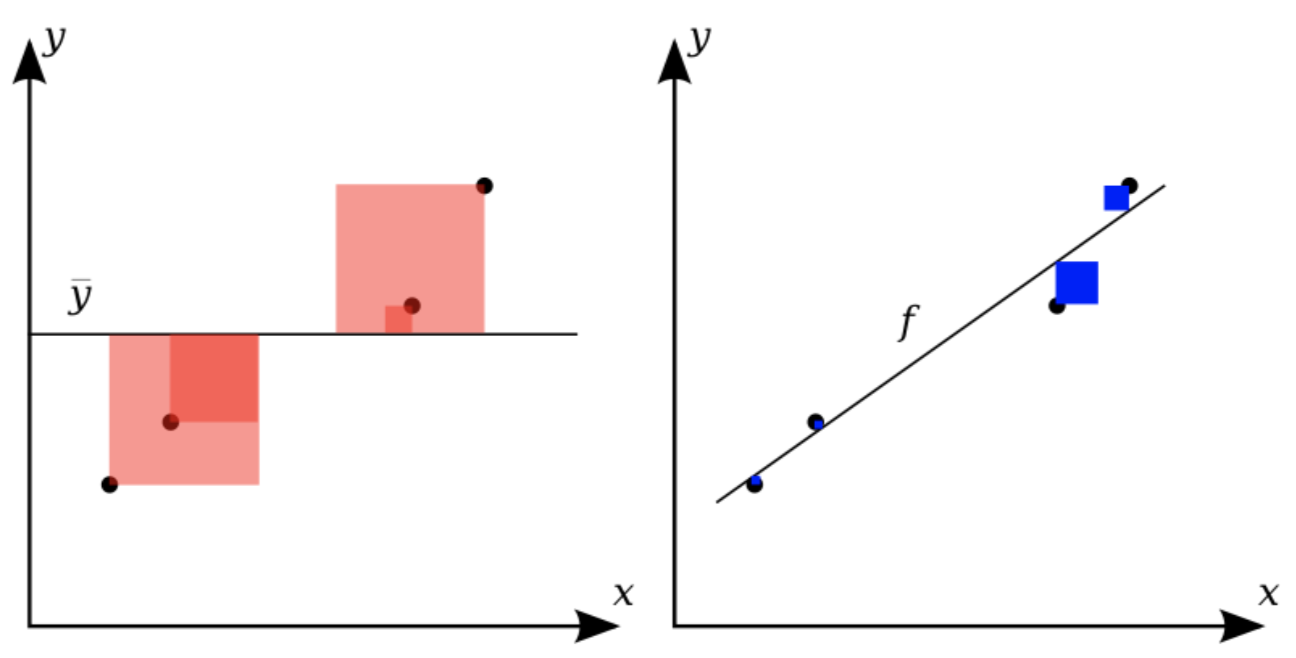
\includegraphics{./Figures/squaredistances.png}
    \caption{Two linear regression taken from two datasets. The left one shows higher square distances than the right one.}
    \label{squaredistances}
\end{figure}

We may note that in some cases, it would be better to rescale the axis to
fit the data with a linear regression. Logarithm axis is the most popular way
of rescaling an axis to have a correct assumption. It is usually more valuable
to rescale the axis and perform a linear regression, than trying to find an
higher order fit.

\section{Linear Regression at Higher Dimensions}

We are now considering higher dimensions data ($p>1$), that are full, meaning
that $p<<N$.
It means that, for an example of data, we might add different parameters. If we
take the example (given in class) of correlations between the velocity of people
versus the size of towns, we might add other relevant parameters, like the
average heigh of people, their ages, etc. We might then examine many potential
predictors. Thus we need to generalise the same things, where each input now
becomes a vector of p dimensions, as presented in equation \ref{pdim}

\begin{equation}
    (x_{i,1}, \cdots , x_{i,p}), \qquad \forall i
    \label{pdim}
\end{equation}

Let now $x_{i,j}$ be the matrix of the input data, where $i$ is the number of
samples, varying from 1 to $N$, and $j$ is the dimension, ranged between 1 to $p$
.

We may generalise the relation $\hat{y_i} = \hat{\alpha} + \hat{\beta}x_i$ in the
new \ref{gen2} equation: 

\begin{equation} 
    \hat{y_i} = \hat{\alpha} + \sum_{j=1}^p \hat{\beta_j} x_{ij}
    \label{gen2}
\end{equation}

If we have this key figure, we can always add 1 in the x vector, as the $p+1$
coordinate. We can thus assume that $\alpha$ vanishes. In fact, we can always
redefine the data so that $\alpha$ vanishes. We can also rescale the variable, by
removing the mean:

\begin{eqnarray}
x’&=& x-\bar{x}\\
y’&=& y-\bar{y}
\end{eqnarray}

Therefore, the output coordinate $\hat{y_i}$ can be written as the product
$\hat{y_i} = X \hat{\beta}$, that is a much more convenient way to write it.

That are just restrictions of the problems that help us to compute it.

Let $l(\beta)$ be the cross-function, define with equation \ref{lbeta}.

\begin{equation}
    l(\beta) = \frac{1}{N} \sum_{i=1}^N \left( y_i - \sum_{j=1}^p \beta_j x_{ij} \right)^2
    \label{lbeta}
\end{equation}

\marginnote{$^T$ denotes the transpose matrix, defined by the relation:
$\left[\mathbf{A}^\mathrm{T}\right]_{ij} = \left[\mathbf{A}\right]_{ji}$}

Let $Z$ be a vector whose components $z_i$ are defined as follows:

\begin{equation}
    \sum_{i=1}^N z_i^2 = ||Z||^2 = Z^TZ
\end{equation}

Therefore we can write the cross-function as:

\begin{equation}
    l(\beta) = \frac{1}{N} (Y-X\beta)^T(Y-X\beta)
\end{equation}

This form can easily be differentiated with $\beta$, and the retrieved derivative
vanishes at the extremum (eq. \ref{lextrem}).

\begin{equation}
    \frac{\partial l}{\partial \beta} =  -\frac{Z}{N} X^T(Y-X\beta) =0
    \label{lextrem}
\end{equation}

The equation \ref{lextrem} can be reduced as $X^TY = X^TX\beta$, which can be
solved by introducing the matrix $C = X^TX$ (eq. \ref{lextremC})\footnote{Note
    that 
\begin{equation*}
C_{ij} = \sum_{k=1}^N x_{kj} x_{ki}
\end{equation*}}

\begin{equation}
    \hat{\beta} = (X^TX)^{-1} X^TY = C^{-1} X^TY
    \label{lextremC}
\end{equation}

At higher dimension, the geometry consists in fitting with an hyperplane, as
shown on figure \ref{hyperplane}.

\begin{marginfigure}
    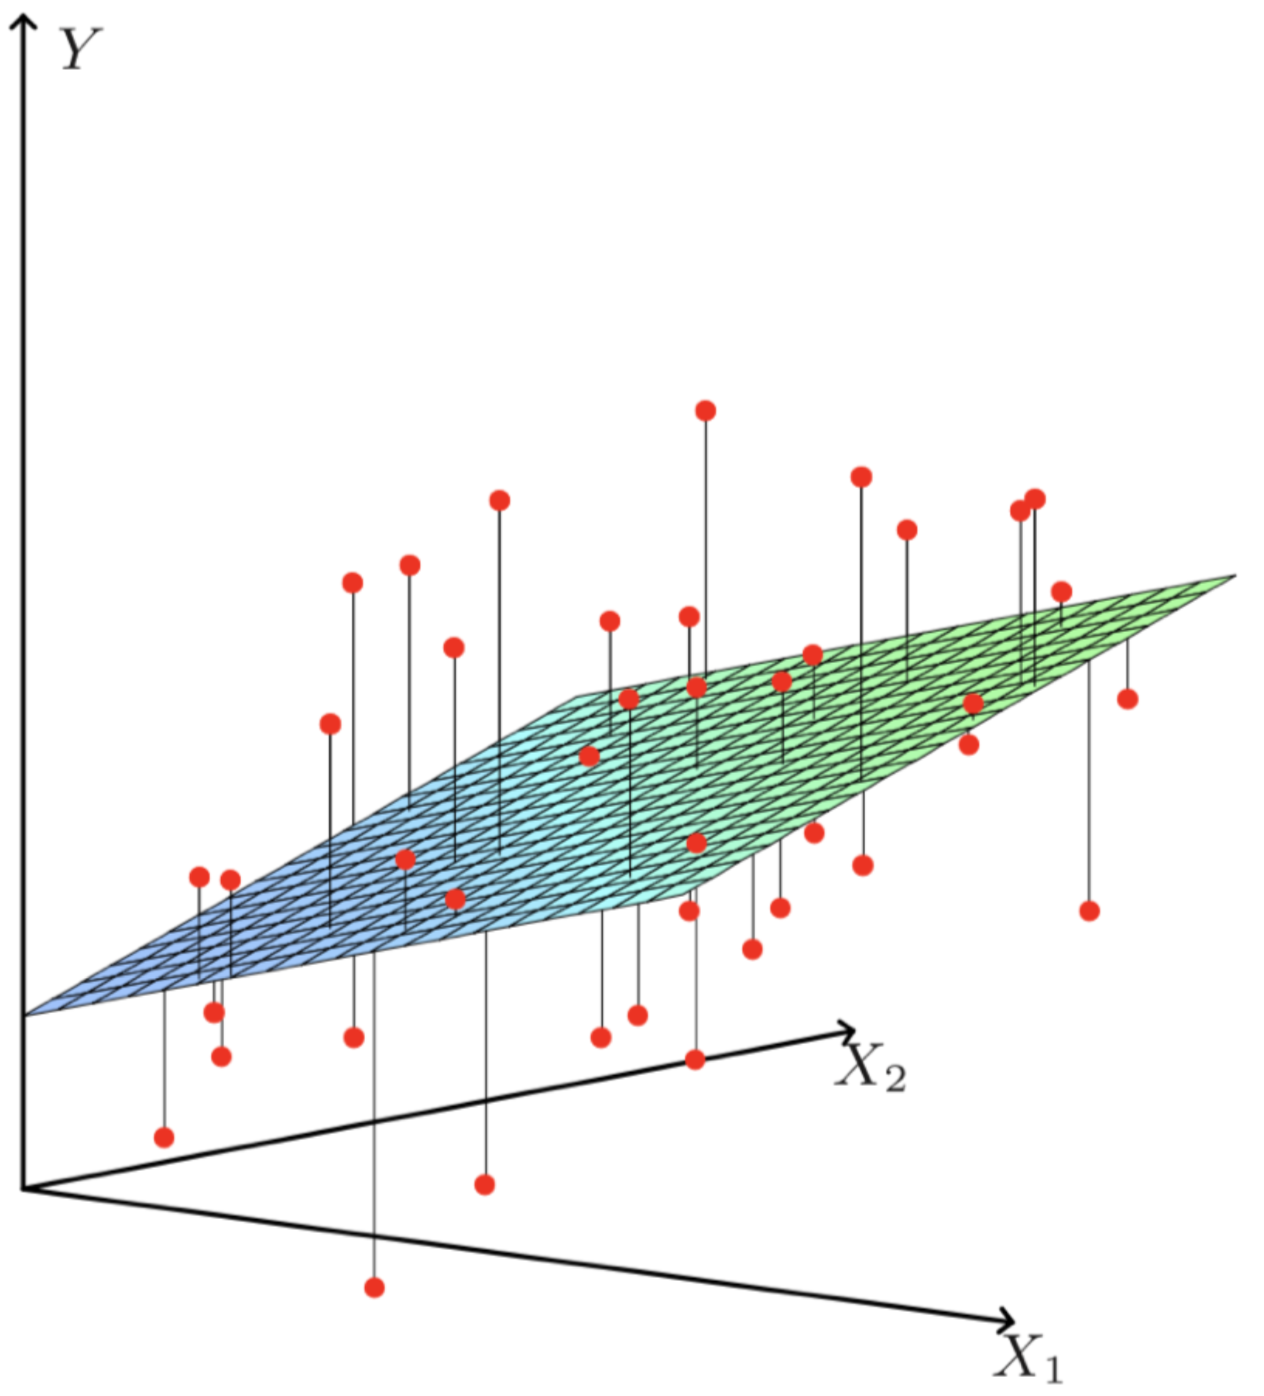
\includegraphics{./Figures/hyperplane.png}
    \caption{Linear least squares fitting with $X\in\mathbb{R}^2$. In this
        problem, we are looking for the linear function of X that minimises the
    sum of squared residuals from Y, which is an plane (hyperplane in dim 3)}
    \label{hyperplane}
\end{marginfigure}

Here, we are essentially solving a system of equations. We must consider the
number of variables adapted to the number of equations that we get. When there is
not enough equations (when $p$ is too small for example), the system is
undetermined. We cannot reduce it and do not have a single solution.

Actually, when $p>N$, we can solve this problem with the condition $\hat{l}=0$.
This is a situation where there are more parameters than there are equaltions. It
is easy to solve. The solutions consists in overfitting.

For instance if we have 100 parameters and 10 equations, we can never manage to
get any result. However, we can find easy solutions, but this will overfit.
At this stage, the system cannot be inverted.

When $p$ is large, even if it is of the same order of magnitude as $N$, we are
working with big matrixes, that can be tricky to invert with both proper
mathematical accuracy and computation performances. In such cases, we should
handle the data carefuly.

Large $p$ are typical way of using statistical learning methods, by
discriminating between datasets without having the aforesaid issues.


\chapter{General principles}
\label{ch:general-principles}

Models, bias vs variance, cross-validation, maximum likelihood, Bayes, etc.


So, what do we do now?
In general, we want to know what are the most interesting parameters. At the end, we can predict the issue with one or two parameters. Even if we spartial with a lot of data, we want to find what are the parameterts, the dimensions important in the problem we are working on.

Two advantages:
\begin{description}
\item[Interpretation]
With less parameters, we can estimate them with much more accuracy than if we have more.
In general, it’s easier and more accurate to estimate things on a condensed set of parameters than on a large set.
The issue is: how do you compromise: having enough parameters to have a good enough estimation of the problem, without having too much and loosing precision. Enough information VS enough precision.
\end{description}

Let $\tilde{l}(\beta)$ be defined as:
\begin{equation}
\tilde{l}(\beta) = l(\beta) + \lambda ||\beta||_q
\end{equation}
With $||\beta||_0 = \#(\beta_j \neq 0)$ (cardinal)

We look for $min_\beta l(\beta)$ given $||\beta||_0 \leq C$

With $\beta = [0, \cdots, \beta_i, 0, \cdots, 0]$
There ain’t any good numerical solution.

There’s always a compromise between what we are able to optimise efficiently, and what is possible to optimise. A version of the problem that is easy to solve is:

\begin{equation}
min_\beta l(\beta)  given ||\beta||_2 \leq C_1
\end{equation}

Ridge regression: there’s a way to get to this problem, using the constraints that can be solved efficiently numerically.

Or $\min_\beta l(\beta)$, given $||\beta||_1 \leq C_2$. This is called the Lasso regression.

In the ridge problem, we assume that the problem is sparse: we only need a few parameters to capture the relationship.

Why did we spartial to write it this way?

\begin{equation}
\tilde{l}(\beta) = (Y -X\beta)^T (Y-X\beta) + \lambda \beta^T \beta
\end{equation}

\begin{equation}
\frac{\partial \tilde{l}(\beta)}{\partial \beta} = 2 (-X^T(Y-X\beta) + \lambda \beta) = 2 (-X^T Y + (X^TX + \lambda \mathcal{1})\beta
\end{equation}

$\mathcal{1}$ is the identity matrix.

What is doing is putting constraints. You add constraints and then you can solve mathematically the problem.

On wenesday, we will compare those two regression, and define the framework for machine learning.

\begin{equation}
C_{jk} \hfill p>N
\end{equation}
\begin{equation}
C_{jk} = \frac{1}{N} \sum_{i=1}^N x_{ij}x_{ik}
\end{equation}

\begin{equation}
\bar{x} = 0 ; C = X^TX
\end{equation}

\begin{equation}
X_{ij} \hfill  Nxp
\end{equation}

$p>N => C$ is non invertible.\\
$N = 1, C_{jk} = x_{1j} x_{1k}$\\
$C = XX^T$ \\
here, $C$ is of rank 1.

NB : remind that $Z^TZ = ||Z||^2$
\begin{equation}
Z^T y = <Z,y> = \vec{Z}\cdot\vec{y}
\end{equation}

Mathematically, $rank(C)\leq N$.
I have too many parametetrs, not enough samples. When I try to solve this linear regression problem, I have too many solutions.

There are issues when p>N, but also when they are of the same order of magnitude.

Example: financial data.

We want to get information from this data, but there’s no label, no y data.
In general, we don’t take the raw data, but try to find something more adapted to the problem.
Here, we want to get rid of the $\alpha$ parameter; for this reason, we use the $r_{ti}$ data instead of the $s_i(t)$ parameter.

Then we define the $x_{ti}$, by substracting the mean and normalising with the standard deviation.

Therefore, the $x_{ti}$ value has a null mean, and a standard deviation rescaled to 1. Therefore each data vary within the same range.

If we move to the data $C_{ij}$

When we have some data, an important step is to watch it by eye, and try to find correlations.
If something is obvious to the eye, we’ll try to interpret it with the math. Example: Exxon\&Chevron are strongly correlated, JP Morgan and Bank of America are also strongly correlated.
Thus, we may suppose that $C_{Ex,Ch} > C_{Ex,JP}$.

In order to analyse the data, we may compute the spectrum. Or see clearly from the definition that the matrix is symmetric, and has all the properties to be diagonalised.

\begin{equation}
C_{jk}, C_{jj} = 1 ; C_{ij} = C_{ji}
\end{equation}

Thus we get $\lambda_1, … , \lambda_p$ eigenvalues, and $v_1, … , v_p$ eigenvectors.

\begin{marginfigure}
\TODO
\caption{dispersion of the eigenvalues}
\label{fig2}
\end{marginfigure}

There’s no way that I can have a good estimation of these metrics.

$Bottom = control$. They just shuffle the data, make permutation of the values. It is the same stocks. Randomy shuffle the data, to remove all the interesting information (correlation between the different stocks).

It’s a way to see what kind of correlation we can get just from randomness, in a case where there’s no corraltion from the data.

We can quantify the quantity of noise.

98\% of the eigenvalues are contained in the 1st partial of the data. That is 98\% of noise.

Therefore I write:
\begin{equation}
C = \sum_{j=1}^p \lambda_j v_j v_j^T
\end{equation} 
\begin{equation}
v_j^T v_k = \delta_j^k
\end{equation}

Random metrics theory: branch of statustical physics, we can compute analytically the shape of the control series. RMT.

$min_x l(x)$ given $g(x)\leq C$\\
$min_x l(x) + \lambda g(x)$  ; $\lambda \geq 0$.

\begin{marginfigure}
\TODO
\caption{scheme}
\label{fig3}
\end{marginfigure}


I assume everything is differentiable.
\begin{equation}
\nabla_x l(x) = -\lambda \nabla_x g(x)
\end{equation}

The conditions tells that the two gradients should be aligned, and directed in opposite directions.
Generally, it would depend on the value C.
Minimum value., can be a local minimum if the problem isn’t perfectly shaped.

If I have $l(\beta)$, and am considering the norm of $\beta$ to be less that C value:
\begin{equation}
||\beta||_q \leq C_q
\end{equation}
We can do it with $l_0$, $l_2$, sometimes also with the $l_1$ norm.

Why are we interested in that kind of things, what does it give us?

With a not too big dataset, taken from a book. The goal here is to try to predict the crime rate, and to what it is correlated.

$(x_{ij}, y_i)$ $i=1..N=50$ cities
$j=1…5$

The idea is to consider naively a simple problem.

Here we may find linear combination of all different problems. For a physicist, it seems we’re not allowed to to so, because not homogeneous. But this helps finding correlations.

$x’_{ij} = x_{ij} - \bar{x_j}$. In this case, we have zero mean, We may also want try to divide by the standard deviation. Not the case here.

\begin{equation}
y=\sum_{j=1}^p \beta_j x_j
\end{equation}

Therefore we can write $l(\beta) = \frac{1}{N} \sum_{i=1}^N (y_i - \sum_{j=1}^p \beta_j x_{ij})^2$

The result of this optimismation may be given as a function.

Graph on the right, ridge regression.
What is plotted is the value of the $\beta$ along the $x$ axis. This has to do with the cost ($c_q$). 
We can repeat for different values of the cost.
If we do it for large $C$, we do not put any constraints, and therefore get the same $\beta$.

if we put a very strong cost, like 0, the only solution is $\beta = 0$.
Hence we’re looking at different solutions, constrained, and then we relax it to a state where there’s no constraint anymore.

The lasso graph is the same, but performed with $l_1$ norm.

There’s a way to understand this, by giving an illustration.

Fig 2.2 slides.


\begin{equation}
y=F(x,\theta).
\end{equation}

Linear models:
\begin{equation}
F(x,\theta) = \sum_{j=1}^p \theta_j x_j
\end{equation}

The principle is to have the results of p data, and then once we get another dataset, similar to the previous one, we’re able to fit it and to find the solution.
\begin{equation}
x_1, \cdots x_p, x_1^2, \cdots, x_p^2, \cdots cos x_1, \cdots
\end{equation}

\begin{equation}
F(x, \theta) = \sum \theta_j h_j(x)
\end{equation}

Later on, we’lll see neural networks. There, the function h people are generally using is:
$h_j(x) = \frac{1}{1 + \exp (-\omega_j^T x )} \omega_j$ is the weight. We’ll see this later.

-> There’s a relation between x and y.
There’s no limit to the complexity of the problem we can take.

Loss function $L (y, F(x, \theta)) = (y-F(x,\theta))^2$.

Training error: $err_{training}$ given a model and given a loss function:
\begin{equation}
err_{training} = \frac{1}{N} \sum_{i=1}^N L (y_i, F(x_i,\theta))
\end{equation}

This is not the only quantity we want to consider.
test/generalisation error. This one would be the error we get when we are using these datapoint that have not been used in the training of the problem.

There’s the training set, used to learn the parameters, and the additional data, on which we’re going to apply the model, and to try to generalise the data that have been used as an input for the fit.

\begin{equation}
Err_{test} = \frac{1}{N’} \sum_{i=1}^{N’} L(y_i’,F(x_i’,\theta))
\end{equation}

Plot in slides: training vs test errors.

The objective is not to get the best fit, but to generalise the given data.

procedure: K-fold cross-validation. 
We would divide the data in 5 datasets, and then, take 1 out to use as the test, and all the other one as training test. 
And then we repeat for all the other combinations. Divide data in K=5 or 10, use most of the data to train, and use one set to test.

Data set is splitted in:
\begin{itemize}
\item training set (for the fit)
\item test set (for model selection)
\item Validation set (for assessment)
\end{itemize}

Typical number would be : 50\%,25\%,25\%.

We use this to understand ho to find the best parameters.

$y=F(x)$

Training set: $\hat{\theta}$

Model $y=F(x,\theta)$

Thus we have $y= \hat{F}(x) = F(x,\theta)$

Another dataset:

$x_0$
\begin{equation}
\E [(F(x_0) - \hat{F}(x_0) )^2]
\end{equation}

Where $\hat(F)$ is the prediction.

This is considered over different training sets. It says how far I am from the value I want to get the prediction.

\begin{equation}
\E[] = F(x_0)^2 - 2F(x_0) \E (\hat{F}(x_0)) + \E (\hat{F}(x_0)^2)
\end{equation}
Where $\E (\hat{F}(x_0)^2)$ is $\var(\hat{F}(x_0) + (\E[\hat{F}(x_0)])^2$

i.e. $\E[] = (F(x_0) - \E[\hat{F}(x_0)]^2 + \var(\hat{F}(x_0))$.

Test error = $(bias)^2$ + variance

We can generalise this when there is some noise $\epsilon$ (random variable) :
\begin{equation}
y = F(x) + \epsilon
\end{equation} 
There we will add another parameter : $var(y)$ that is irreducible error.

In the context of linear regression, there’s the Gauss-Markov theorem.
It tells us that in linear regression, all the estimators that have no bias, the best one is the one that is minimising the loss function
\begin{equation}
L(y,F(x)) = (y-F(x))^2
\end{equation}
This theorem is telling us that if we’re interesting in minimising the bias in the context of linear regression we should take $min_\beta l(\beta)$

No bias + min var => $min_\beta l(\beta)$.
In general, the best solution is not the solution that has no bias.
I will estimate better the parameters that I have with a constrained set of data.


\chapter{Supervised learning: classificaton, regression, nearest neighbours}
\label{ch:supervised-learning}

last time, we learnt unsupervised learning.
$(x,y)_{i=1\cdots N}$

Goal : learn $x \rightarrow y$. function: theta
so that when given new $x_i$

$x_i \rightarrow^{predict} \hat{y_i} \sim y_i$
function: $\hat\theta$


function with two components : $err_{test}$ wich is composed of the bias +
variance.
if large amount of data, high variance, very hard to learn, and we get
very different parameters.

we may want to compromise this with a model with less parameters with 
a lower variance problem.
not only we want to pick the best variable in the model, but also the model
itself.
we consider a class of problems, described with a parameter $\lambda$.
we introduce $\lambda$ as a parameter of regularisation.

\marginnotes{we are difining, for example, the error as:
\begin{equation*}
    l(\beta,\lambda) = \frac{1}{N}\sum_{i=1}^N (y_i - \beta x_i)^2 - \lambda ||\beta||_0
\end{equation*}
}

\begin{itemize}
\item training -> $\hat \theta$ given $\lambda$
\item validation -> $\hat \lambda$
\item test -> $Err_{test}$
\end{itemize}

At the begining, we divide the dataset into multiple datasetts.

K-fold cross validation : the idea is that we have one dataset, that we divide
into K subsets. We can get it with statistics. two weeks ago, we've seen an example of this, in the context of linear regression.
minimising the mean square error

planning of the day:
\begin{itemize}
\item Bayesian approach
\item how we do the approximation in practice.
\item example of CLASSIFICATION.
\end{itemize}

First, let's discuss about maximum likelihood estimation.
This is not a big-data specific approach. general in statistics.
In general, I would have a model of the form $ y= f(x,\theta)+ \epsilon$
where $\epsilon$ stands for the noise. it is a random variable.
We suppose $\epsilon$ is a normal variable:
$\epsilon \~ N(0,\sigma^2)$

The probability to see x with theta:
\begin{equation}
P(y|x,\theta) = \frac{1}{\sqrt{2\pi\sigma^2}} \exp - \frac{(y-f(x,\theta))^2}{2\simga^2}
\end{equation}

\begin{marginfigure}
\TODO
\caption{P(y|x,theta) representation. with the standard deviation $\sigma^2$ and centered on f(x,theta)}
\label{gauss}
\end{marginfigure}

Now, let's imagine we are given a set of values $(x_i,y_i)$. We want to find
the best parameter $\hat \theta$.
We look at the parameter that make the data the most likeable.

\begin{eqnarray}
\mathcal{L} (\theta|\Z_1,\cdots,Z_n) & =&  \log P(Z^N|\theta)\\
& = & \sum_{i=1}^N \log P(Z_i|\theta)\\
&=& \sum_{i=1}^N \left[ -\half \log (2\pi\sigma^2) - \frac{1}{2\sigma^2} (y_i - f(x_i,\theta))^2 \right]\\
& = & - \frac{N}{2} \log(2\pi\sigma^2) - \frac{1}{2\sigma^2} \sum_{i=1}{N} (y_i -f(x_i,\theta))^2 \\
&=& -\frac{N}{2} \log(2\pi\sigma^2) - \frac{1}{2\sigma^2} l(\theta)
\end{eqnarray}

MSE

MLE: $max_\theta \mathcal{L}(\theta,Z^N) \rightarrow \hat\theta$
theorem:
if $y =f(x,\theta_0) + \epsilon$
$$\E[\hat\theta] \rightarrow_{N\rightarrow\infty} \theta_0$$
$$\hat\theta \~ N(\theta_0, F(\theta_0)^{-1})$$

$F(\theta) = \E\mathcal{L}(\theta)$ this is called the Fisher information.

$I(\theta)_{ij} = - \frac{\partial^2 \mathcal{L}}{\partial \theta_j \partial\theta_k}$

Therefore,

$\hat\theta \sim (approx) N(\hat\theta, I(\hat\theta)^{-1})$

\begin{marginfigure}
\TODO
figure parabolle inversée, maximum : courbature $-\partial\mathcal L/\partial \theta^2$, absisse max : $\theta_0$. ordonnée : L.
\end{marginfigure}

We want to find the best parameter, \ie the one that is the more likelihood to be \ldots

L is called the log-likelihood. P is colled the likelihood.
In a sense, we want to find the most likely model.

We can mention, that there are two difficulties :
\begin{itemize}
\item we need to find the maximum
\item problem of validation: if we have a more complicated model, we would increase the log likelihood, and no way to do the validation.
\end{itemize}

Now, another approach: the Bayesian approach. Again, this is not specific to big-data.
We may know that there are lot of debates in the meaning of probabilities. There
are two schools: the frequentists: probabilities have a meaning only when the
event is reapeating many times. Like a coin tail or head. Fundamentally, if I do
it a large number of time, this is converging.
If we take an event that can happen only once: the probability that there's lifeon the moon: for a frequentist, there's no meaning.
the Bayesian view is different in nature: probability is not about counting, but
about biliefs. This represent how I believe the event to be actually the case.
Concretely, the idea of the bayesian approach is:
elementary probability: when I have two random variables X, Y.
The joint probability of (X,Y): P(X,Y). we can also define the marginals :
$P(X)$, $P(Y)$, that are only the probability $P(X) = \sum_y P(X,Y)$.
$P(X|Y)$: conditional probability.
$P(X,Y) = P(X|Y)P(Y)$
therefore $P(X|Y) = \frac{P(X,Y)}{P(Y)}$.


$P(Z,\theta) = \frac{P(Z,\theta)}{P(Z)} = \frac{P(Z|\teta)P(\theta)}{P(Z)}$.
This is called the Bayes formula.

$P(Z=1) = \theta$
$P(Z=0) = 1-\theta$, for example, for a binomial problem.

$P(Z|\theta)$ is the likelihood I had before.
In this approach, there's something new, that is $P(\theta)$ wich is called the prior.
For a bayesian, we always have some \emph{a priori} bieliefs about the
distribution of the parameters. When I see the data, I have to update my
beliefs.
$P(\theta|Z)$ is called the posterior.
$P(Z)$ is called the evidence.

Here we have to do the inference, that is the general model. Usually, when we
look at probabilites, we look at $P(Z|\theta)$. reverse approach.
We look at  the model, that also incorporates the prior.

On the slides, one partialicular example of the prior to solve a praticular problem.


Here, there's nothing to do with big data. example taken from the book of MacKay
example: Jo has a test for a disease. a = state of health.
a=1 if sick, 0 otherwise.
the test is giving another variable b
what is known about this test is that it can be positive even if there's no
disease. $P(b=1|a=1) = 95\%$. same for zero.
it means the test gives the right result in 95\% of the cases.
we need to know the case when somebody of HIS AGE has the disease. this
is gonna be the prior. $P(a=1) = 1\%$.
The exercise is to find what is the probability $P(a=1|b=1)$.
In the bayesian approach, we do not have a theta, but a distribution of the theta
we always have a probability to have different values, especially the maximum
\emph{a posteriori} estimate (MAP)
which is given by taking the max of this:
$\max_\theta P(\theta|Z)$.

It will give the same results if we are assuming that this is not depending on theta. If we have a flat prior.
Then, this is equivalent to the MLE.

When I'm maximising the posterior, it means I'm maximising the likelihood.
Thus we can see the likelihood as a bayesian approach, with a partialicular prior
value.

Let's say we have the same model as before. This time, we assume the prior is
a one dimensional variable, with a gaussian distribution.

$f(\theta)  = \sqrt{\frac{\lambda}{2\pi}} e^{-\lambda \frac{\theta^2}{2}}$

Then, this will be very similar to the l validation, if we take the log of this.
Then, this is multiplied by lambda theta square over two.

When we take a prior on these parameters, we want to give more probability to
the small values of the parameters. width of the gaussian: 1/sqrt(lambda).
control the probability of the parameter to have a large value.
restricting the range of the parameter that we are considering, as we saw before

The goal here is to present this partialicular approach, and recover the maximum
likelihood.
An interesting aspect of the bayesian approach. Again, this is very general.
Let's say that, in general, we have the probability of the data, given some
hypotheses:

$P(D|H_1)$
Dis the data, $H_1$ thehypothesis.

we want to compare with another hypothesis: $P(D|H_2)$

What the bayesian approach is telling us is that we have to consider the
probability :
$\frac{P(H_1|D)}{P(H_2|D)} = \frac{P(D|H_1)P(H_1)}{P(D|H_2)P(H_2)}$

it depends on the prior we put there. we do not here have no belief????

One example of the maximum likelihood and the general approach.

Problem of generalization.
Let's say we have the data:
$x_{i=1\ldotsN}$. two approaches are possible:
MLE that gives $\hat\theta$
bayesian that gives $P(\theta|X)$.

what is the probability of a partialicular value?

$P(x_{N+1}) = $(MLE) $P(x_{N+1}|\hat\theta)$. if we need a best value of approximation, let's replace the parameter.

= (bayesian)$ P(x_{N+1} | X^N) = \sum_\theta P(x_{N+1}|\theta P(\theta |x^N)$

here, $P(\theta |x^N)$ should be used as the new prior. We are constantely updating our believes. this is the prior we get before knowing the
value,
depending on what we saw before. This has to be equal to:
$\frac{P(x^N|\theta)P(\theta)}{P(x^N)}$

There's a famous problem that has to do with that: the rule of succession.
The sun is rising every morning, what is the probability it will rise tomorrow?
Laplace discussed this issue.

With different approaches, we may get different results. One of the simplest
example.
Let's assume there's some probability $\theta$ the sun is rising in the morning.
We hae a binomial model. This is the same issue as a coin that always ends up
in the same edge: tail for example.
Maximum likelihood estimation: the probability would be 1.

$x_i = 0/1.$

$x^N = (x_1, \ldots ,x_N) = (1,\ldots,1)$

$P(x_{N+1} = 1) = ?$
If we do the maximum likelihood approximation, this would be 1 everytime.

$X^N : N_1 times 1 ; N-N_1 times 0.$ (times : frequency it happens over time)

$P(x_i|theta) = \theta$. One parameter model, binomial model.
Obviously, the probability $P(x_i=0|\theta) = 1 - \theta$. this example cannot be
simpler than this.


theta can be anything between 0 and 1. $0 \leq \theta \leq 1$.

I'm giving the same probability for every $\theta$. $P(\theta)\~ $uniform.

$P(x_{N+1} =1|x^N) = \int d\theta P(x_{N+1}=1|\theta) P(\theta|x^N)$
$= \int d\theta \theta \frac{P(x^N|theta)P(\theta)}{P(x^N)} where P(\theta) = 1$
$= \frac{N!}{N_1!(N-N_1)!} \theta^{N_1} (1-\theta)^{N-N_1}$

The difficulty lies in the $P(x^N)$ that does not depend on theta.

$P(\theta|x^N)=C(N,N_1) \theta^{N_1} (1-\theta)^{N-N_1}$

$\int d\theta P(\theta|x^N) = 1$

$\int_0^1 d\theta \theta^a (1-\theta)^b = \frac{a!b!}{(a+b+1)!}$
this exists also for a and b that are not integer values, and this is called the
gamma function.
If we use this formula, we would find this to be:

$c(N,N_1) = \frac{(N+1)!}{N_1!(N-N_1)!}$
with the proper normalisation.
I need just one line to compute the stuff.
If I compute this:

$P(x_{N+1}=1|x^N) = \int_0^1 d\theta \theta \frac{(N+1)!}{N_1!(N-N_1)!} \theta^{N_1} (1 - \theta)^{N-N_1}
= \frac{(N+1)!}{N_1!(N-N_1)!} \frac{(N_1 + 1)! (N-N_1)!}{(N+2)!}
= \frac{N_1 + 1}{N+2} \neq \frac{N_1}{N} (MLE)$

this is called as the laplacian formula.

we have a non-zero probability to observe something that we have never observed
before.

$N=3. X^N = (1,1,1). can we bet that x_4 = 1?$
maybe it is not very wise to say this. this rule takes this into account. here, the probability to be 0 will be 1/5, not zero.

people that carry out statistics use pseudo-counts. we are adding one zero and one one.
It is a way to regularise the variation.
In this case, a frequentist would say that we have too few points and that we
must give up the problem. for a bayesian, the calculation would be very
dependant on the prior.
Prediction on the next outcomes.

commentary:
$I(\theta) = -\frac{\partial^2 \mathcal{L}}{\partial \theta_i \partial \theta_j}$

$\mathcal{F} (\theta) = \E [I(\theta)]$
MLE: $\hat\theta \~N(\ldots)$
For each dataset, we can use another expectation. It is mathematical consideration,
considering all the possibilities of my data.If we arepartialificially generating
data 
when we want to prove all mathematical results analytically, we need all the
possible datasets that we can get.
variance about everything we can get when generating different datasets.







second hour.



Now I want to discuss the computational issues.

$\hat \theta$ that I want to maximise. 
log likelihood: $\mathcal{L}(\theta|x^N)$. we would have, in general, to get these
data numerically, and not analytically, with optimised function. compromises to
be done.

Very simple, but the problem can be complicated if the function has several minimum.
Let's assume the problem is convex: the function is convex, as well as the set
of data.
Any global minimum is a global minimum. It can be generate, but,\ldots

In all these problems, we can consider a gradient descent.

If we want to minimise the function,

scheme fig 2.
If we look at the gradient, and spartial from a point (random). we look at the
grandient, and move in the direction of it.
we usually take a very small displacement. spartial iteratively.

$\theta_{t+1} = \theta_{t} - \eta \left( \frac{\partial L}{\partial \theta}\right)_{\theta_{t}}$

scheme: cf notes.

cf learning rate, etc.

$L(\theta) = \sum_{i=1}^N (y_i - f(x_i,\theta))^2
= \sum L_i(\theta)$.
for each calculation, we have to recompute the data.
a version of this algorithm is used very often, and is called stochastic gradient.
What we do is: compute $L_i(\theta)$ for a subset of the points.
So we take a subset of samples to estimate $L(\theta) = \sum_{i\in subset}$ and we
change at each iteration.
The sample is called mini-batch.

There's one version of this algorithm, where everytime we take a single value as
a subset: subset =1. this is called on-line learning. in this case, what we are
doing is:

$\theta_{t+1} = \theta_{t} - \eta \nabla_\theta L_i(\theta_{t})$.

The issue is to get faster. In general, we have to take the sum.
At the end, it is equivalent to do a move at everytime than getting the sum from
the very beginning.
Actually ,this algorithm is very powerful. In neural networks, backpropagation
is nothing more than this algorithm put in application.

This is really a local method. If I spartial from one point, I can end somewhere
different. I can be trapped in local minima. It is really difficult to find the 
correct minimum. That's why we usually work with convex functions, where local
minima do not exist elswhere than the global minimum.

$l_0$ norm, $l_1$ norm.
$||\beta||_0 = \# nonzero \beta_j ; ||\beta||_1 = \sum_j |\beta|_j$

For this reason the closest problem to the first is with $l_1$, and it is convex
so that it can be solved with an iterative method. Generally, these are
considerations we want to take into account.
We will see examples of doing this next time.

Next week: exercise as homework. practical.
that will be the grade.

$min_\beta L(\beta) -> \hat \beta$

Lasso regression.
this is one in which we are going to impose a condition:
$||\beta|| \leq t$
this is equivalent to the fact that we want to minimize :
$min_\beta L(\beta) + \lambda ||\beta|| with some parameter \lambda.$

ridge regression: $||\beta|| = ||\beta||_2^2
= \sum \beta_i^2$

if we take the $l_1$ norm:

lasso regression: $||\beta|| = ||beta||_1 = \sum |\beta_i|$

At this stage, we can take it as an exercise.

Le'ts spartial with the function I want to minimize.
$\mathcal{L} (\beta) = \frac{1}{N} \sum_{i=1}^N (y_i - \beta x_i)^2 + \lambda |\beta|$

differentiation: we must be careful.

$\frac{\partial\mathcal{L}}{\partial\beta} = 0$

the maximum, if $\beta$ is positive ,let's say, we can get the value:
$(\beta >0)$

$\frac{\partial\mathcal{L}}{\partial\beta} = - \frac{2}{N} \sum_{i=1}^N (y_i - \beta x_i)x_i + \lambda.$

I would take $\bar{x} =0, \bar{y} = 0$ and $\overline{x^2} = 1$. normalise all the
data.

In general, everything can have completely different units. It makes sense here
to normalise, so that each data has the same range of variation.
So

$dL/d beta = -2 (\frac{X^T y}{N} - \beta) + \lambda = 0$

thus $\hat \beta = \frac{X^Ty}{N}- \frac{\lambda}{2}$

If $\frac{X^Ty}{N} > \frac{\lambda}{2}$, thus
$\hat{\beta} = \frac{X^Ty}{N} - \frac{\lambda}{2} >0$

if $\beta < 0$, then we can use the same approach.

$\hat \beta= S_{\lambda/2} \left( \frac{X^T y}{N} \right)$

$S_a (u) = \sign(u) \max(O,|u|-a)$. soft-thresholding operator. cf figure notes.

This is a figure for p=1.

cf on the website a slide with the formulas.

for $p>1$,

$L(\beta) = \frac{1}{N} \sum_i (y_i - \sum_k \beta_k x_{ik} )^2 + \lambda \sum_k |\beta_k|$

$= \frac{1}{N} \sum_i (y_i - \beta_j x_{ij} - \sum_{k\neq j} \beta_k x_{ik} )^2 + \lambda |\beta_j| + \lambda \sum_{k\neq j} |\beta_k|$

let's define $r_{ij} = y_j - \sum_{k\neq j} \beta_k x_{ik}$
$\hat{\beta_j} <- S_{lambda/2} (\frac{1}{N} x_j^T r_j)$
cyclical coordinate descent. we do this for j, and then repeat for j + 1 until
convergenc.
we get an interative algorithm. $\beta_1$, then $\beta_2$, \ldots

Because the truc is convex, this is going to converge to the minimum of the function $L(\beta)$.

cf note on this algorithm. If we understand the case for p=1, then we repeat,
and because the problem is convex, we're going to converge to the single minimum.

On wednesday, we will see single classification.

\chapter{Unsupervised learning: dimensionality reduction, PCA, SVD}
\label{ch:unsupervised-1}

regression = supervised learning for quantitative data.

$x->y$

if we want to classify pictures between cats and dogs, two kinds of methods:
- supervised: give information before
- unsupervised: you figure out that there are two categories, understand that
there are two categories, and learn from that.

fig 5

distincition on the nature of the variable that we want to predict.
quantitative data : why is it a real number or a vector?

we are going to see today classification. so far we've seen just supervised
quantitative : regression. there are more task to do.

today : classification.
next course : clustering.
after that : neural networks, that can be used for any of those tasks, that
involve a bit more methodology.

CLASSIFICATION. 

training data: $(x_i,k_i)$

label : $k_i = 1, 2, \ldots K$.



Again, the challenge is using large datasets. we use big data.
$x_{N+1} \rightarrow^? k_{N+1}$

so far we've used only regression.
if we start with only two categories : $K=2$.
$k_i \in \{ 0, 1 \}$

from these data, I can try to predict the value of K in unsupervised learning.
the closest to 0 and 1, and then get a classification.

let's start with the case where $p=1$.
fig 6

we have to find a value somewhere to split the value between two sets of data.
generally, we have more complicated problems, in larger dimensions.
here, if we do a linear regression:

$y = \hat \alpha + \hat \beta x$.
this is what we did in the first lecture: compute $\hat \alpha$ and $\hat \beta$ that gave us
the best result.

decision boundary:
$if \hat y is larger than \half, then \hat k = 1$.

$\hat y < \half => \hat k = 0$

if we start again with p=2.
it can be in two dimensions.

fig 7.

data linearly separable: we can put an hyperplan that separates the data.
define a decision boundary.
there we can define an error.

NB: in advance, we cannot preduct wich method would work, before looking at the
data. In practical, no method would separate perfeclty the data.
if we augment the dimension of the space, we can consider other functions : for
example quadratic instead of linear.
tradeoff : if we add more parameters, sure we can reduce the training error, but
also, in general, increase the variance.
back to the problem already discussed: how to find the correct level of
complexity. surely it can fit the data, but may not be generalised.

data still have to be linearly separable.
again we'll se a second class of methods. ability to solve different issues.
fig 8 for example (marginfigure)

now, let's add another data.
if $y= 0,1,2$, there is no practical meaning. no classical order. here it is
classification.
it works well with two categories. if we have three categories, then we can
split between two categories. data: 1 VS 1.
based on the boundaries, I will decide which boundary I can consider.


This was a naive approach. If I start again with p=1:
fig 9.

we added data far enough to put the blue squares in another category.

linear regression:

\begin{equation}
    \min_\beta \frac{1}{N} \sum_i (y_i - \beta x_i)^2
\end{equation}

it is more convenient to work with more symmetric data.
the problem with saying that the error for i is:

\begin{equation}
    error_i = (y_i - \beta x_i)^2.
\end{equation}

$K=2$: $k_i = \pm 1 bd$ if $\hat \beta x >0 => +1$
$if \hat \beta x<0 => -1$

what matters is wether the quantity $\hat y = \hat \beta x$ has the correct sign
or not.

\begin{equation}
    L(\beta) = \frac{1}{N} \sum_i \max(0, -y_i\beta^T x_i)
\end{equation}

here again, the idea is that when $\beta x$ is of the same sign as $y$, the maximum
is zero, and the error is zero.

this is called hinge regression.

the idea is gradient descent

smooth version -> logistic regression.

the idea is to replace this versiona
fig 10.
\begin{equation}
    L(\beta) = \frac{1}{N} \sum_i \ln (1+e^{-y_i \beta^T x_i )
\end{equation}

he tries to minimise the error, and the split value with  that logistic regression.

we can also arrive to similar results by chosing different approaches.
this is connected to the kind of operations that are done in neural networks.
we will see this later on.

instead of taking the reflection y to be k, it's easier to consider y to be
a probability. it makes here much more sense to make a linear regression.
a probabilistic model, in which I want to describe the probability, given some data.
parameter $\omega$: weight, standard notation in neural networks, whereas $\beta$ is
much more used in classical regression/statistical learning models.

\begin{equation}
    P(k=1 | x,\omega)
\end{equation}

\begin{eqnarray}
    P(k=1|x,\omega ) & > &  P(k=-1|x,\omega) & => \hat k = 1 \\
    & < &     &  => \hat k = -1
\end{eqnarray}


if we are considering the log of the proabilities:
\begin{eqnarray}
    \ln \frac{P(k=1|x,\omega)}{P(k=-1|x,\omega)} & = & \omega^T x\\
    & = &  \sum_{j=1}^P \omega_j x_j (+\omega_0)
\end{eqnarray}


I don't have to always write $+\omega_0$, for convenience, just changes in the
problem that have no influence.

In general, I want to define a more relevant model.

Let's call:
\begin{equation}
    y=P(k=1|x,\omega)
\end{equation}
\begin{equation}
    \ln (\frac{y}{1-y}) = \omega^T x
\end{equation}

\begin{equation}
    \frac{y}{1-y} = \exp (\omega^T x)
\end{equation}

thus
\begin{equation}
    y = e^{\omega^T x} (1-y)
\end{equation}

therefore
\begin{equation}
    y(1+e^{\omega^T x}) = e^{\omega^T x}
\end{equation}

\begin{equation}
    y = \frac{e^{\omega^T x}}{1+e^{\omega^Tx}} = \frac{1}{1+e^{-\omega^T x}}
\end{equation}

\begin{equation}
    P(k|x,\omega) = \frac{1}{1+e^{-k\omega^T x}}
\end{equation}


\begin{equation}
    \mathcal{L}(\omega) = \frac{1}{N} \sum_i \ln P(k_i |x_i,\omega) MLE
\end{equation}

if i replace P by its form:

\begin{equation}
    \mathcal{L}(\omega) = - \frac{1}{N} \sum_i \ln (1 + e^{-k_i \omega^T x_i})
\end{equation}

Essentially, the idea was to apply the maximum likelihood. I had to make 
hypothesis on the general form of the model. Once I do this, I
end up with this function. The different with the one above:  minus sign.
not surprising: a likelihood we want to maximise, and not error we want to
minimize.

\begin{equation}
    \max_\omega \mathcal{L}(\omega) <=> \min_\beta L(\beta)
\end{equation}

in neural networks,

fig11

\begin{equation}
    u = \sum_{j=1}^p \omega_j x_j = \omega^T x 
\end{equation}
is called the activation.

several inputs, and one output based on this.
if $u>0$, then I have output $y=1$.
if $u<0$, then $y=0$.

in the context of neural networks, people prefer work with 0 and 1 rather than
$\pm 1$.

neuron is a classifier

fig11

\begin{equation}
    y = \phi (u)
\end{equation}

\begin{equation}
    \phi (u) = \frac{1}{1+e^{-u}}
\end{equation}

essentially, what we do, is considering the different inputs with different
weights.
At the end, we will end with more complex classifier models. this one is very
elementary.
there are very simple algorithms, like the gradient descent.


let's start again with the log likelihood:

\begin{eqnarray}
    \mathcal{L}(\omega) & = & \frac{1}{N} \sum_i (k_i \ln y_i + (1-k_i) \ln(1-y_i))\\
    & = & \frac{1}{N} \sum_i \ln P (k_i | x_i,\omega)
\end{eqnarray}

\begin{equation}
    y_i = P(k_i =1 |x,\omega)
\end{equation}

\begin{eqnarray}
    ln(P(\ldots)) & = & y_i & if k_i = 1 \\
    & = & 1-y_i & if k_i = 0
\end{eqnarray}

then we make the model by assuming:

\begin{equation}
    y_i = \phi (u_i) where u_i = \omega^T x_i = \sum_{j=1} \omega_j x_{ij}
\end{equation}

now, we want to compute the gradient.
it means to compute the derivative of the log likelihood:

\begin{equation}
    \frac{\partial \mathcal{L}}{\partial \omega_j} = \frac{1}{N} \sum_i (k_i \frac{1}{y_i} \frac{\partial y_i}{\partial\omega_j} - (1-k_i)
\frac{1}{1-y_i}) \frac{\partial y_i}{\partial \omega_j}
\end{equation}

with
\begin{equation}
    (\ldots) = \frac{ k_i (1-y_i) - (1-k_i)y_i}{y_i (1-y_i)} = \frac{k_i - y_i}{y_i (1-y_i)} 
\end{equation}


and \begin{equation}
    \frac{\partial y_i}{\partial \omega_j} = \phi'(u_i) \frac{\partial u_i}{\partial \omega_j} = \phi'(u_i) X_{ij}
\end{equation}


thus
\begin{equation}
    \frac{\partial \mathcal{L}}{\partial\omega_j} = \frac{1}{N} \sum_i \frac{\phi'(u_i)}{\phi(u_i) (1-\phi(u_i))} (k_i - y_i) x_{ij}
\end{equation}

\begin{equation}
    \phi (u) = \frac{1}{1+e^{-u}} => \frac{\phi''}{\phi (1-\phi)} = 1
\end{equation}

\begin{equation}
    \frac{\partial \mathcal{L}}{\partial \omega_j} = \frac{1}{N} \sum_i (k_i - y_i) x_{ij}
\end{equation}

for neural networks, the same idea as gradinet descent is called backpropagation
, but it is a bit more complicated.

fig 2.1: representation of classification.

support vector machine : SVM
problem formally attitred: 
\begin{equation}
    \min_\omega \sum_i \max(0,1-k_i \omega^T x_i ) + \lambda ||\omega||^2
\end{equation}

the exercise is trying to find what this function is doing.

standard linear regression: take care about the distance to the line.
when doing SVM: introducing some margin of errors.
this approach would count as an error even if we are on the right side of the
line but close to it.
we're not going to explain it here, but it looks very much linke the other frameworks.

another approach:
linear discriminant analysis (LDA)

we take a model (probabilistic), more gaussian like. the objective function is
to fit two classes by the gaussian, in such a way we maximise the distance
between the gaussians, and minimise the variance of the gaussians.
that can easily be done with linear algebra.

there are many other methods on the same lines.

Now we want to be able to adress the problem of non linear separability.
where the real boundary would be a circle.
in and out.

fig12

we can also do this locally.

it is called k-nearest neighbours

again, let's start with a batch of values:
fig13

we are given with a particular point, and say if it is red or blue.
what are the neighbours doing?

if $k=3$, i am looking at the three nearest points, and then take the colour of
the majority.

mathematically, it can be written as:

\begin{equation}
    \hat y(x)  = \frac{1}{k} \sum_{i\in N_k(x)} y_i
\end{equation}


$N_k(x)$ is the set of $k$ nearest neighbours to $x$

$y_i \in \{0,1\}$

Again, we can be in a situation described by fig 14.
we have, there, a decision boundary. i'm deciding what is the coulour of the
nearest points with that boundary.

fig 2.2 and 2.3. variations of K

now the question is: what should we take for K

$\frac{N}{k} \sim p$ : number of degrees of freedom.


fig 15

figure slide: 'selection of K': using 10,000 datapoints and tested with 200.

minimal training error if we take k=1. very complicated thing.
as we are taking larger and larger values of k, we are averaging and get more
errors, even in the training set.
if we have too few degrees of freedom, we are completely missing the structure
of data.
it is also not good if we have too many degrees of freedom.

15 is relatively well located in this area.
between 20 and 10, there's not that much difference, maybe 10 is better
because it uses less resources.
we have to pick the right model, and there are models of different levels of
complexity.
different values of k that can be used.

there is nothing into this algorithm, but also nothing trivial in finding the right datapoints.

there are many variations along this method.
in this example, we are taking the same density of points, everywhere. but if I take any point, it doesn't mean anything to take just three points
randomly.
we may take into account the distance between the points.
essentially, we would average around the point that are close to the considered
point. more generally, we can do it with a hard cutoff close/far or smooth
cutoffs.

\begin{equation}
    \hat y(x) = \frac{\sum_i K_\lambda (x,x_i)y_i}{\sum_i k_\lambda (x,x_i)}
\end{equation}

\begin{equation}
    K_\lambda (x,x_i) = \frac{1}{\lambda} e^{-\frac{||x-x'||^2}{2\lambda}}
\end{equation}

or $K_\lambda (x,x_i) = 1$ if $||x-x'||<\lambda$, 0 otherwise.

kernel methods also posisble.
if we do this, it is also a case where we have one parameter: $\lambda$. It plays
the same role.
big lambda: averaging a lot.
we would reduce the variance, but with a too large bias.
in the opposite: reduce the bias would end in a too large variance.

again, there are variety of methods that can be used. one way to see this
problem of classification is to fit a function.
let's say, zero for orange points, 1 for blue points.

At one dimension, we would have
fig 16.

maybe there could be errorsa

the thing is that we may smooth all those functinos.
we may think about these problems as fitting problems. correcting locally
the errors of the functions.

kernel method smoothing, to locally have something smoother.
what these things are doing is similar to the problem of smoothly inferring a
function from just any perfect observation.

This is very simple, but the problem is that none of those things are working
for big data. issue of classifying dogs and cats.

If we go in any of those methods, there is no way we can succeed. Several
problems, the greatest is a geometrical one:
the curse of dimensionality.

essentially, it has to do with all the assumption we have about neighbourhoods
are false when we are working with high dimensional spaces.

example in 2D in fig 17.

volume is scaling as power p of the radius. $V = \alpha_p r^p$.

If we look at $\frac{V}{V_{tot}} = \left( \frac{r}{r_{tot}} \right)^p$

then we have 

\begin{equation}
    \frac{r}{r_{tot}} = \left( \frac{V}{V_{tot}} \right)^{1/p}
\end{equation}


If the ratio V/Vtot = 0.01.
if we take something like p=10, we'll see that r/rtot = 0.6.

if we want to cover even a very small fraction of the volume, we have to go very
far from the point.
ridiculous amount of the volume.
the problem of scaling with the radius is not interesting.
in high dimensional spaces, all the volume is close to the centre.

to cover a small fraction of the volume, we have to go very far.

All the ideas of closest neighhbourgs cannot be used in high dimensionality
spaces.

we can also reduce the dimensionality of the data. that is the first approach
with this problem.
solutions:
\begin{itemize}
    \item reduce dimensionality -> PCA (unsupervised)
    \item representation, that has to do with what kind of space we are woking with. we have to imagine that we have all the pictures of cats and
        dogs, all put in the same place.
        something invariant with translation, rotation, etc. so this will be seen in another lecture, about neural networks. essentially, one
        class of netwkrs: convolutional, is based on this. chose the right space
        in which it is easy to chose the classification.
\end{itemize}

exam
In priciple, everything should be comprised in the lecture.
code it ourself. not using things already written. the game here is to write
ourself our own libraries. it is not very complicated, each question is just
a few lines of code.

with python: using the jupyter.
matlab: not sure it is doeable. livescripts.
write a report in which he can see the code. in a format he can actually work
the code.
minimal thing: write the code and display the figures.
this is a public problem, neither on the solutions presented on the internet is
good, we might think about it from ourselves.





\chapter{Unsupervised learning: clustering, K-means, hierarchical}
\label{ch:unsupervised-2}

\chapter{Neural networks, from single neuron to multilayer networks}
\label{ch:neural-networks}

\chapter{Physics of machine learning, statistical mechanics of machine learning, applications}
\label{ch:physics}

\end{document}
